\documentclass[11pt]{article}
\usepackage[margin=1in]{geometry}
\usepackage{graphicx}
\usepackage{amsmath}
\usepackage{amssymb}
\usepackage{xcolor}
\usepackage{hyperref}

\graphicspath{{figures/}}

\newcommand{\fd}{\phi_{\rm FD}}
\newcommand{\Iobs}{I_{\rm obs}}
\newcommand{\Qobs}{Q_{\rm obs}}
\newcommand{\Uobs}{U_{\rm obs}}

\title{Faraday rotation with the LuSEE-Night four-port correlator:\\
  zoom-bin spectroscopy of the polarized sky}
\author{}
\date{\today}

\begin{document}
\maketitle

\begin{abstract}
We redo the LuSEE-Night Faraday-rotation forecast on the full
four-port instrument model, producing all sixteen correlation products
of the N, E, S, W monopoles, and propagate them through the actual
spectrometer channelization, including the 64 zoom sub-bins of the
25\,kHz parent channels.  A single fully polarized source behind a
$\fd = 250\;{\rm rad\,m^{-2}}$ screen produces polarization
oscillations with a $\sim$1.9\,kHz period at 30\,MHz: erased to
better than $10^{-3}$ in the parent channels, but recovered at
$\sim$79--86\% amplitude by the zoom bins (with a zenith-calibrated
four-port polarimeter whose instrumental leakage is nulled exactly).  [Steps 2--4: realistic
sky, 10/50\,MHz bands, delay-space signature -- to be filled in.]
\end{abstract}

\section{Simulation setup}
\label{sec:setup}

The instrument model is the luseepy four-port response (BGL\_v16 v3
artifact): coupled $2\times$ monopole fields $H^{\theta,\phi}_p$ for
the ports $p \in \{{\rm N,E,S,W}\}$, antenna impedance matrix $Z_A$
and the JFET receiver loading $M = Z_L (Z_A + Z_L)^{-1}$.  For a sky
coherency written in the tangent basis $(e_\theta, e_\phi)$ of the
topocentric frame,
\begin{equation}
  B_E = \frac{k_B \eta_0}{\lambda^2}
  \begin{pmatrix} I + Q & U - jV \\ U + jV & I - Q \end{pmatrix},
\end{equation}
the open-circuit pair correlations are beam-weighted integrals of the
pair-Stokes kernels $P^{I,Q,U,V}_{ab}$, and the loaded covariance is
$C = M K M^\dagger$.  The sixteen telemetered products are the four
autos and the real/imaginary parts of the six crosses.

The analysis band is a $\pm 0.1$\,MHz window around a band center
$\nu_0 \in \{30, 10, 50\}$\,MHz, sampled by a fine grid of
$16384$ frequencies spaced at $25\,{\rm kHz}/2048 = 12.2$\,Hz.  The
beam is deliberately frozen at the native $\nu_0$ channel (the
fixed-beam approximation), so that any spectral structure is purely
the Faraday phase
\begin{equation}
  (Q + iU)(\nu) = (Q + iU)\, e^{+2 i \fd \lambda^2(\nu)} .
\end{equation}
Time is sampled at 1024 points over exactly one lunar sidereal day
(27.32\,d), making the time axis periodic and FFT-ready.  The
observatory is at the LuSEE-Night site
($-23.814^\circ$, $182.258^\circ$).

The fine waterfalls (time $\times$ frequency $\times$ 16 products) are
integrated against the measured spectrometer response into (i) the
three 25\,kHz parent channels covered by the window, (ii) their
$3 \times 64$ zoom sub-bins (390.625\,Hz spacing, FFT ordering), and
(iii) an idealized set of Gaussian zoom bins of matching FWHM at the
nominal sub-bin centers.

The pixel-space engine was validated against the luseepy harmonic
engines: point-source covariances agree with
\texttt{FullStokesCalibratorSimulator} to $9\times10^{-16}$ relative,
and the diffuse-sky transport (frame rotation, polarization spin,
COSMO/IAU conventions, absolute normalization) against
\texttt{FullStokesCroSimulator}.

\section{Step 0: an unpolarized source and the calibrated polarimeter}
\label{sec:unpol}

We first characterize the instrument itself on a transiting
\emph{unpolarized} point source (1\,K\,sr), placed so that it
culminates $0.6^\circ$ from zenith; it is above the horizon 56\% of
the sidereal day.  With the frozen beam and no polarization the
response is exactly frequency-flat — parent bins, zoom bins and fine
channels are identical — so any recovered pseudo-polarization is
pure instrumental leakage.  Figure~\ref{fig:ionlysource} shows this
leakage as a function of source altitude for the raw
$X = {\rm E{-}W}$, $Y = {\rm N{-}S}$ polarimeter: an ideal
crossed-dipole polarimeter would give zero leakage at zenith, but
the as-built four-port beams retain $p \simeq 0.13$ even at transit,
rising to $\simeq 0.94$ at $30^\circ$--$35^\circ$ altitude.

\begin{figure}[htb]
  \centering
  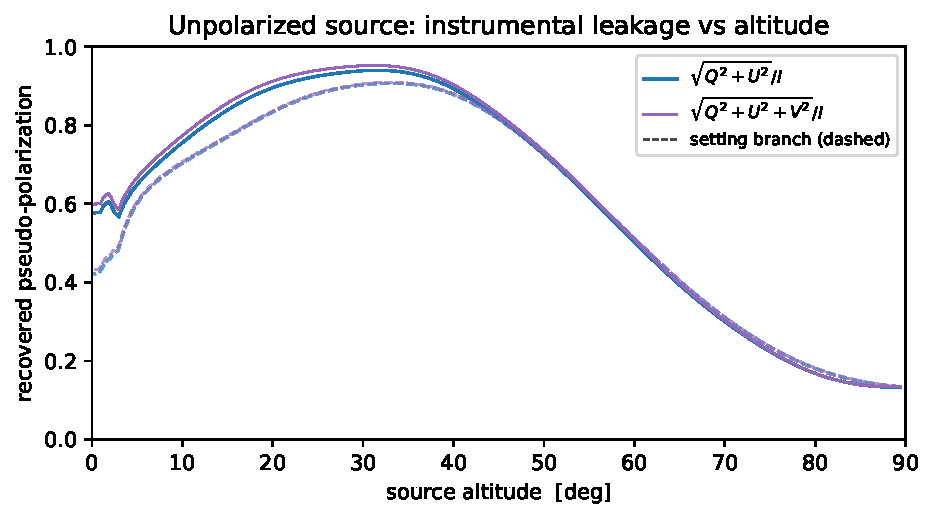
\includegraphics[width=0.85\textwidth]{step1_ionly_polfrac}
  \caption{Unpolarized transiting source, \emph{raw}
    $X = {\rm E{-}W}$, $Y = {\rm N{-}S}$ polarimeter: the recovered
    pseudo-polarization is pure instrumental leakage (frequency-flat,
    so all channelizations coincide).  Solid: rising branch, dashed:
    setting branch.}
  \label{fig:ionlysource}
\end{figure}

\paragraph{Zenith-calibrated polarimeter.}
The zenith leakage reflects the asymmetry of the as-built beams: an
unpolarized source at exact zenith produces autos
$(NN, EE, SS, WW) \propto (1.26, 1.12, 1.25, 1.00)$ and the raw
polarimeter reports $(q, u, v) = (-0.094, -0.096, +0.013)$.  We
calibrate the polarimeter on this zenith response in two stages.
First, per-port gain weights $X = w_E E - w_W W$,
$Y = w_N N - w_S S$ with $w_p \propto C_{pp}^{-1/2}$, i.e.\
$(w_N, w_E, w_S, w_W) = (0.952, 1.019, 0.956, 1.079)$ (plus a common
$X/Y$ rescaling), null the zenith pseudo-$Q$ exactly but leave
$u = -0.096$: that term enters through the inter-port
cross-couplings ($\langle N E^* \rangle$ etc.) in
$\langle Y X^* \rangle$ and no real per-port gain can touch it.
Second, we therefore let $X$ and $Y$ be \emph{complex combinations of
all four ports}: the zenith conditions $Q = U = V = 0$ for pure $I$
are precisely the statement that $x$ and $y$ are orthogonal with
equal norms in the metric of the zenith covariance $C_0$, so a
symmetric (L\"owdin) $G^{-1/2}$ orthonormalization of the
gain-weighted pair achieves them exactly while staying as close as
possible to the E--W / N--S dipoles.  The result,
\begin{align}
  X &= 1.023\,E - 1.082\,W + (0.046 + 0.004i)(N - S),\nonumber\\
  Y &= 0.955\,N - 0.959\,S + (0.049 - 0.004i)\,E
      - (0.052 - 0.004i)\,W,\nonumber
\end{align}
leaves zenith leakage of $(q, u, v) \sim 10^{-16}$ — zero to machine
precision.  Figure~\ref{fig:ionlycal} repeats the unpolarized track
with these vectors: the transit leakage collapses from 0.134 to
$7\times10^{-4}$ (set only by the source culminating $0.6^\circ$ off
exact zenith).  Away from zenith the leakage is essentially
unchanged — the calibration enforces a single condition at one
direction — so compact-source polarimetry remains leakage-limited at
low altitude.  All polarimeter results in the remainder of this
report use the calibrated vectors; the raw-polarimeter figure
versions (step1\_* instead of step1w\_* in
\texttt{report/figures}) are retained for reference.

\begin{figure}[htb]
  \centering
  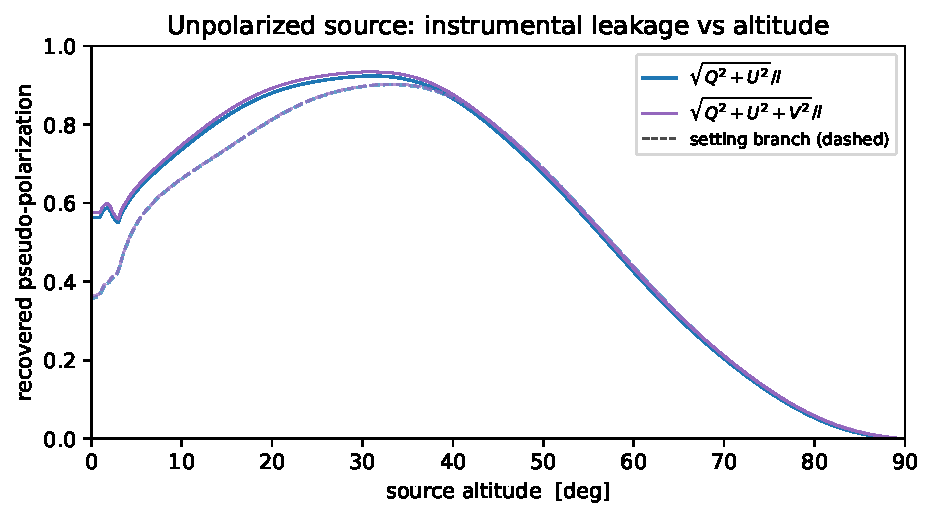
\includegraphics[width=0.85\textwidth]{step1w_ionly_polfrac}
  \caption{As Fig.~\ref{fig:ionlysource}, with the zenith-calibrated
    four-port polarimeter.  The leakage now vanishes towards transit
    ($p \to 7\times10^{-4}$ at $0.6^\circ$ from zenith), while
    remaining $O(1)$ at low altitudes where the single-point zenith
    calibration has no power.}
  \label{fig:ionlycal}
\end{figure}

\section{Step 1: a single polarized source}
\label{sec:point}

The same transiting source, now fully polarized with its electric
vector fixed along ecliptic north.  The instrument-frame polarization
angle is $\chi(t, \nu) = \psi(t) + \fd \lambda^2(\nu)$ with $\psi$
the parallactic angle and $\fd = 250\;{\rm rad\,m^{-2}}$.  All
pseudo-Stokes below use the zenith-calibrated polarimeter of
Sec.~\ref{sec:unpol}.

At 30\,MHz the Faraday oscillation period is
$\Delta\nu = \pi \nu_0^3 / (2 \fd c^2) \simeq 1.9$\,kHz
(Fig.~\ref{fig:transit}): about 13 full $Q \to U \to Q$ rotations fit
inside one 25\,kHz parent channel, while a zoom bin samples only
$\sim 0.2$ of a rotation.  Figure~\ref{fig:transitzoom} zooms into
$\pm 3$\,kHz of the same spectrum, where the individual oscillations
and the amplitude transfer of the real and ideal zoom bins are
visible.  The recovered polarization fraction of every frequency bin
at transit is collected in Fig.~\ref{fig:polfracbins}, and
Fig.~\ref{fig:polfractrack} follows it along the whole track as a
function of source altitude.  Finally, Fig.~\ref{fig:xycoherency}
shows the four correlator combinations of the calibrated polarimeter
— $\langle|X|^2\rangle$, $\langle|Y|^2\rangle$,
${\rm Re}\,\langle XY^*\rangle$, ${\rm Im}\,\langle XY^*\rangle$ —
as waterfalls over the track; the full set of sixteen raw N/E/S/W
products is available as the step1\_product\_waterfalls figure in
\texttt{report/figures}.

\begin{figure}[htb]
  \centering
  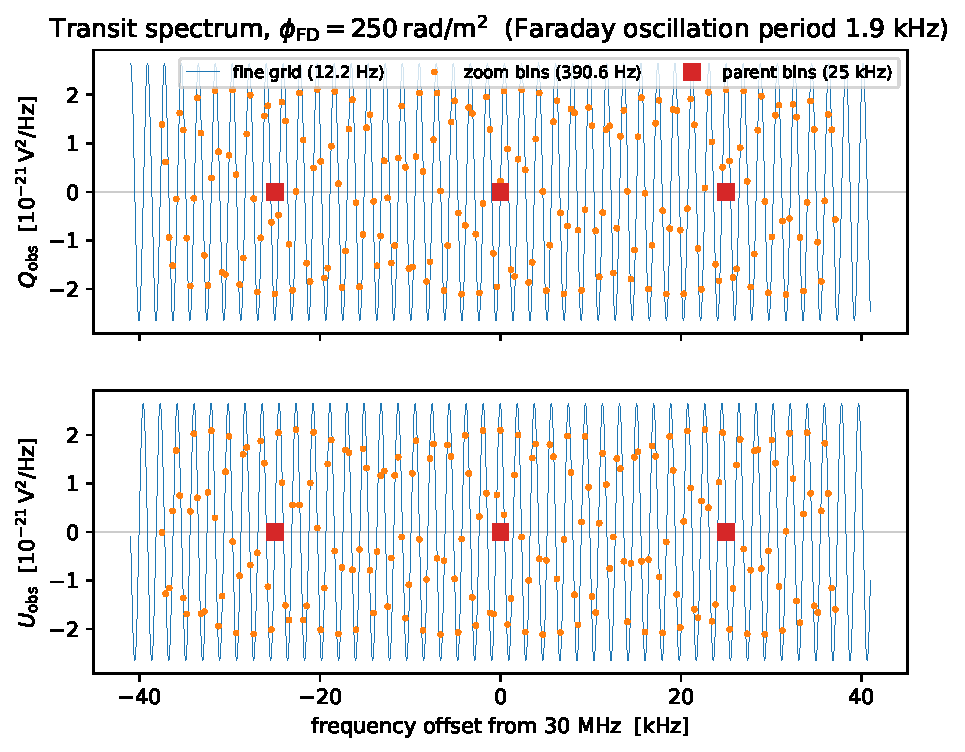
\includegraphics[width=0.95\textwidth]{step1w_transit_spectrum}
  \caption{Observed pseudo-Stokes $\Qobs$, $\Uobs$ (zenith-calibrated
    polarimeter) at transit as a function of
    frequency.  The fine grid (blue) resolves the 1.9\,kHz Faraday
    oscillation; the zoom bins (orange) trace it with a mild amplitude
    suppression; the parent 25\,kHz bins (red) are almost completely
    depolarized.}
  \label{fig:transit}
\end{figure}

\begin{figure}[htb]
  \centering
  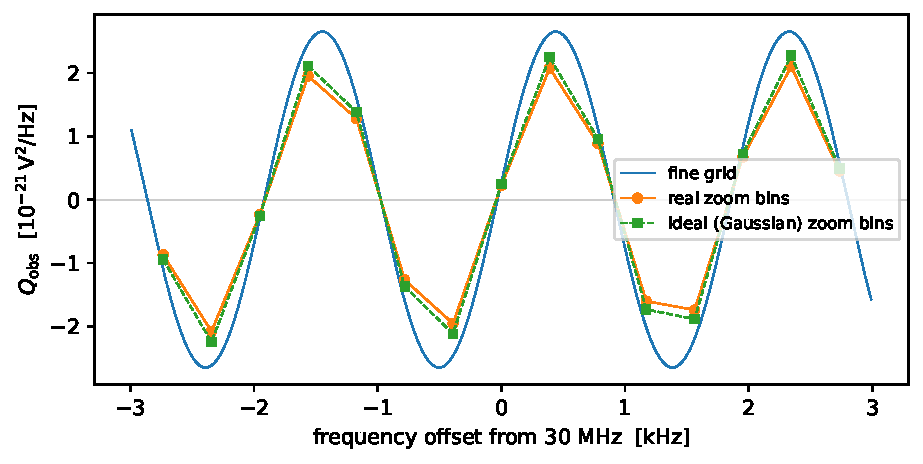
\includegraphics[width=0.8\textwidth]{step1w_transit_spectrum_zoom}
  \caption{Zoom into $\pm 3$\,kHz around the band center.  Real
    (measured response) and ideal (Gaussian) zoom bins track the fine
    spectrum with $\simeq 0.79$ and $\simeq 0.86$ of the amplitude
    respectively.}
  \label{fig:transitzoom}
\end{figure}

\begin{figure}[htb]
  \centering
  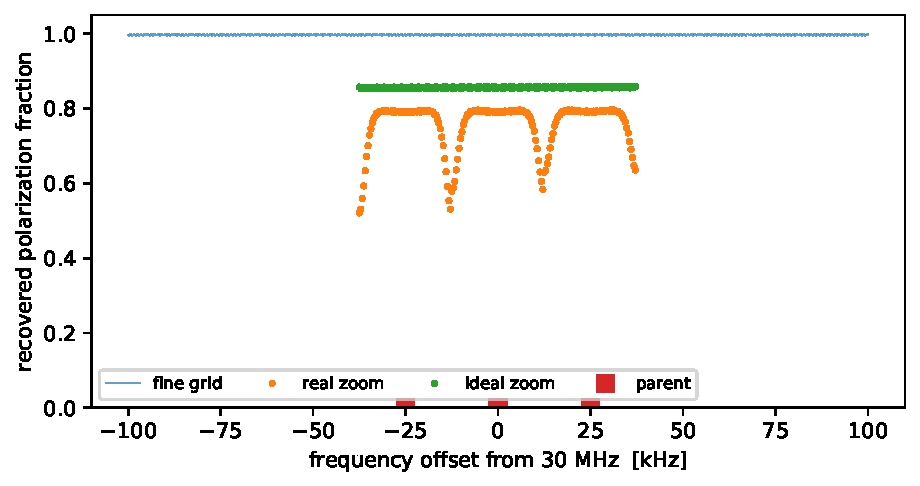
\includegraphics[width=0.85\textwidth]{step1w_polfrac_bins}
  \caption{Recovered polarization fraction at transit per frequency
    bin.  The fine grid sits at $p \simeq 1$ (rank-1 source); with
    the leakage nulled, the parent channels now show the true
    bandwidth depolarization, $p \simeq 7\times10^{-4}$; ideal zoom
    bins recover a flat $p \simeq 0.86$, while the real zoom bins
    (median 0.79) show characteristic dips at the parent-bin edges
    and centers caused by their aliased response tails.}
  \label{fig:polfracbins}
\end{figure}

\begin{figure}[htb]
  \centering
  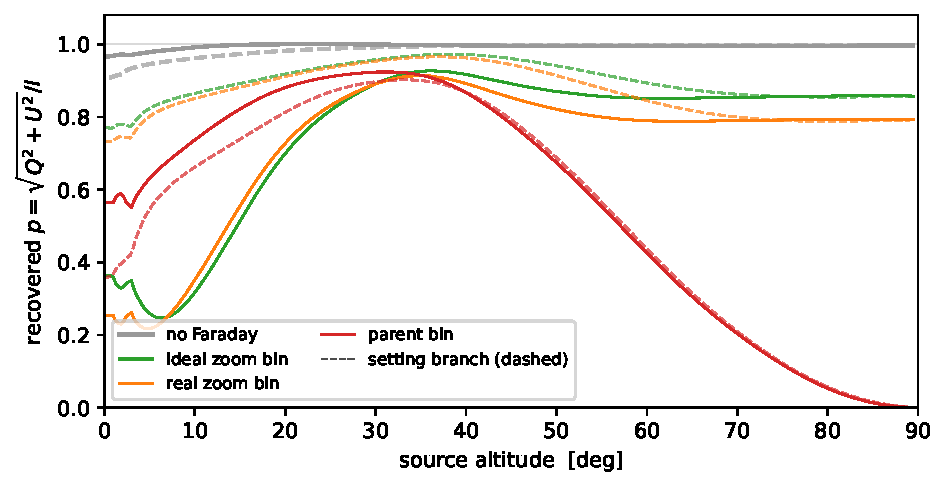
\includegraphics[width=0.85\textwidth]{step1w_polfrac_track}
  \caption{Recovered polarization fraction as a function of source
    altitude (solid: rising branch, dashed: setting branch; the two
    differ because the parallactic angle, and hence the
    instrument-frame EVPA, is not symmetric about transit).  The
    fully polarized source has a rank-1 covariance, so
    $p \le 1$ always, with the Faraday-free curve (grey) saturating
    the bound at essentially all altitudes.  The 25\,kHz parent bins
    (red) depolarize essentially completely near transit
    ($p \to 7\times10^{-4}$), where the intrinsic $\sim$1.9\,kHz
    Faraday oscillation dominates the bin average; the residual floor
    equals the calibrated leakage of Fig.~\ref{fig:ionlycal}, since a
    fully depolarized bin leaves exactly the unpolarized-source
    covariance.  Towards the horizon the parent bins recover more
    polarization while the zoom bins lose some, as beam-phase
    gradients across the bin become the limiting factor.}
  \label{fig:polfractrack}
\end{figure}

\begin{figure}[htb]
  \centering
  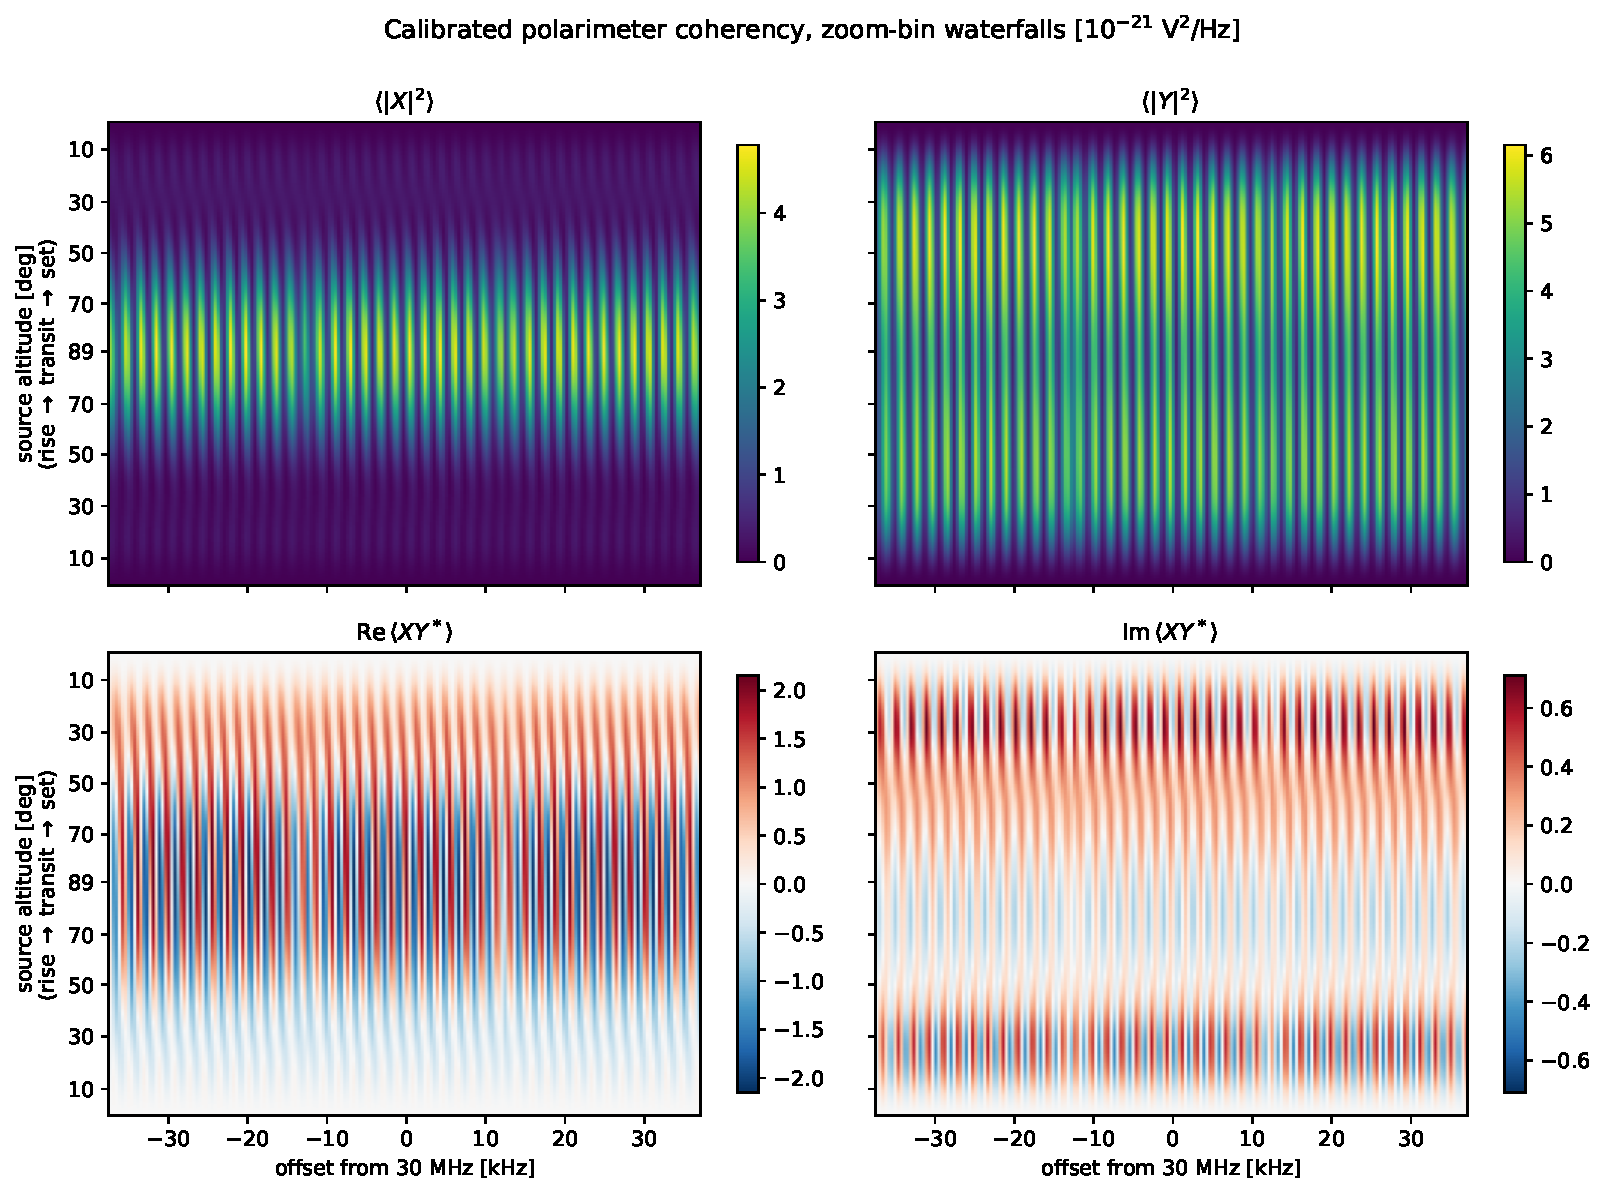
\includegraphics[width=\textwidth]{step1w_xy_waterfalls}
  \caption{Coherency of the zenith-calibrated polarimeter in the
    zoom-bin channelization, against source altitude along the track
    (rise $\to$ transit $\to$ set) vs.\ zoom frequency:
    $\langle|X|^2\rangle$, $\langle|Y|^2\rangle$ (top) and
    ${\rm Re}\,\langle XY^*\rangle$, ${\rm Im}\,\langle XY^*\rangle$
    (bottom), where $X$ and $Y$ are the calibrated four-port
    combinations of Sec.~\ref{sec:unpol}.  The 1.9\,kHz Faraday
    oscillation appears as vertical striping in all four panels; the
    slow structure along the track is the parallactic rotation of the
    source EVPA (which moves power between the $X$ and $Y$ autos)
    modulated by the altitude dependence of the beam.}
  \label{fig:xycoherency}
\end{figure}

\section{Step 2: the real sky at 30 MHz}
\label{sec:realsky}

The sky model (Fig.~\ref{fig:skymodel}) combines the destriped,
desourced Haslam 408\,MHz map scaled with $\beta = -2.55$ for $I$, the
WMAP K-band (23\,GHz) $Q,U$ maps scaled with $\beta = -2.8$, and the
Hutschenreuter \& En{\ss}lin (2020) mean Faraday-depth sky.  All maps
are used at their native $N_{\rm side} = 512$: the per-pixel Faraday
phase does not commute with pixel-averaging, so the maps are never
degraded; the pixel-space engine sums the full-resolution maps
directly.  Here and in everything that follows, the pseudo-Stokes are
formed with the zenith-calibrated polarimeter of
Sec.~\ref{sec:unpol}, using the weights of the respective band
center.

\begin{figure}[htb]
  \centering
  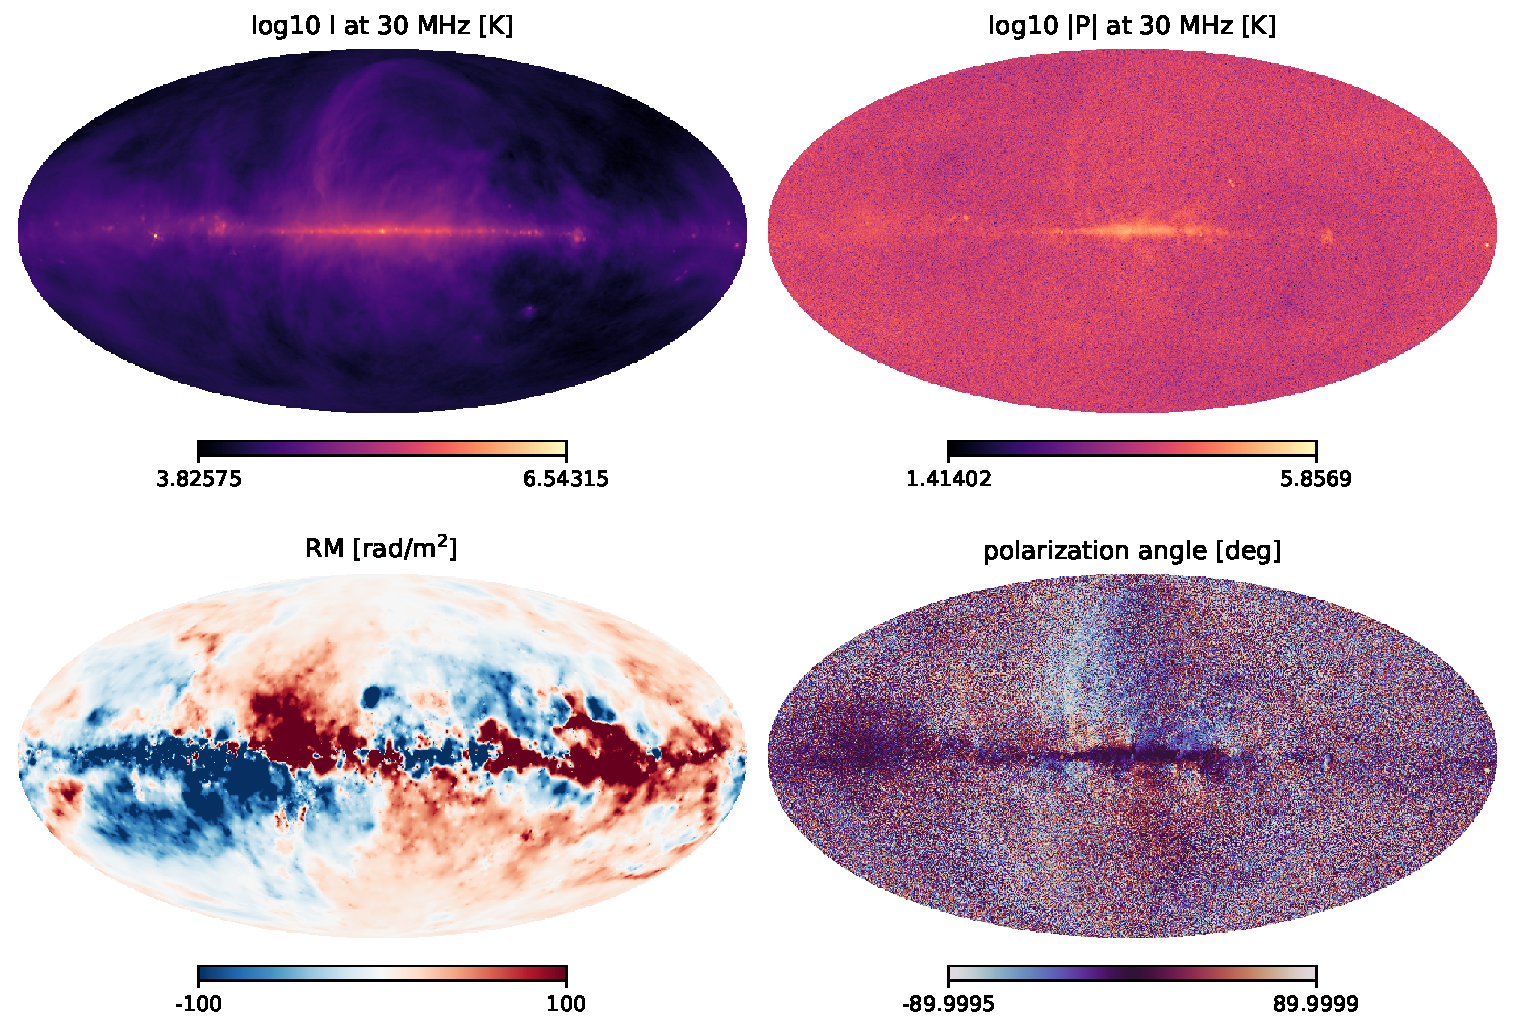
\includegraphics[width=\textwidth]{real30_sky_model}
  \caption{Input sky at 30\,MHz: intensity, polarized intensity,
    Faraday depth and polarization angle (native
    $N_{\rm side}=512$).}
  \label{fig:skymodel}
\end{figure}

\begin{figure}[htb]
  \centering
  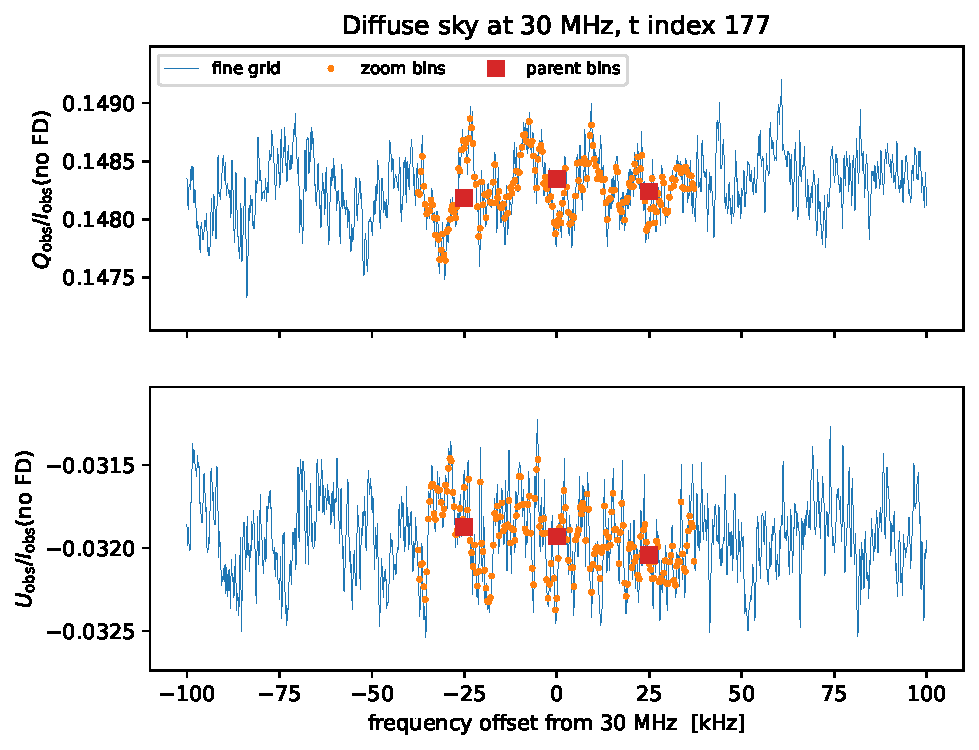
\includegraphics[width=0.9\textwidth]{real30_spectrum_snapshot}
  \caption{Beam-integrated $\Qobs/\Iobs$, $\Uobs/\Iobs$ across the
    $\pm 100$\,kHz window at the time of maximum sky signal, with the
    y-range zoomed onto the fine-grid structure (the Faraday-free
    level lies far off scale).  The smooth mean level is almost
    entirely instrumental leakage of the \emph{unpolarized} emission
    (Sec.~\ref{sec:ionly}); the fast ``hash'' riding on it, at the
    few$\times10^{-3}$ relative level, is the surviving sky
    polarization scrambled by the many rotation measures within the
    beam.  The zoom bins trace a smoothed version of the hash while
    the parent bins average over it.}
  \label{fig:realsnapshot}
\end{figure}

\begin{figure}[htb]
  \centering
  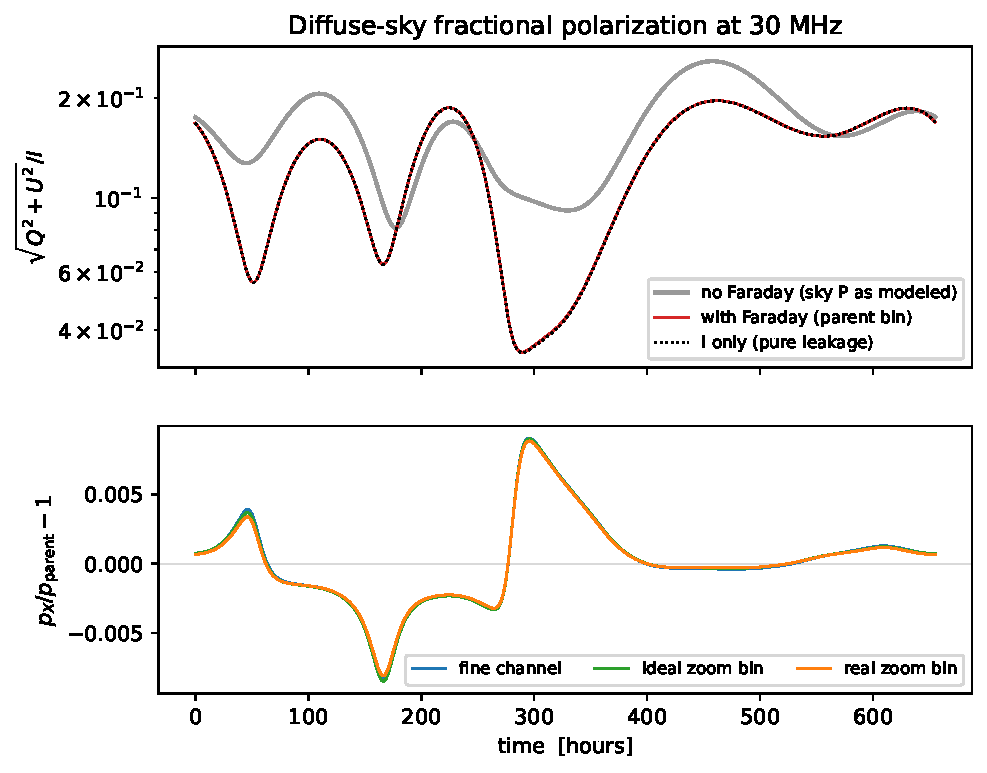
\includegraphics[width=0.85\textwidth]{real30_polfrac_track}
  \caption{Fractional polarization of the beam-integrated signal over
    one sidereal day.  Top: ``no Faraday'' keeps the sky polarization
    exactly as modeled (WMAP-scaled $Q,U$) with the Faraday screen
    switched off; ``with Faraday'' is the full simulation in the
    central parent bin; the dotted line is the $Q = U = 0$ (I-only)
    run, i.e.\ pure instrumental leakage.  The Faraday curve lies
    exactly on the leakage curve — after beam-scale rotation-measure
    scrambling, the recovered polarization \emph{is} the leakage
    track (cf.\ Sec.~\ref{sec:ionly}).  Bottom: fine-channel,
    ideal-zoom and real-zoom values relative to the parent bin — all
    channelizations agree to better than 1\%: at 30\,MHz the
    diffuse-sky spectral structure is resolved even by the 25\,kHz
    parent bins.}
  \label{fig:realpolfrac}
\end{figure}

\begin{figure}[htb]
  \centering
  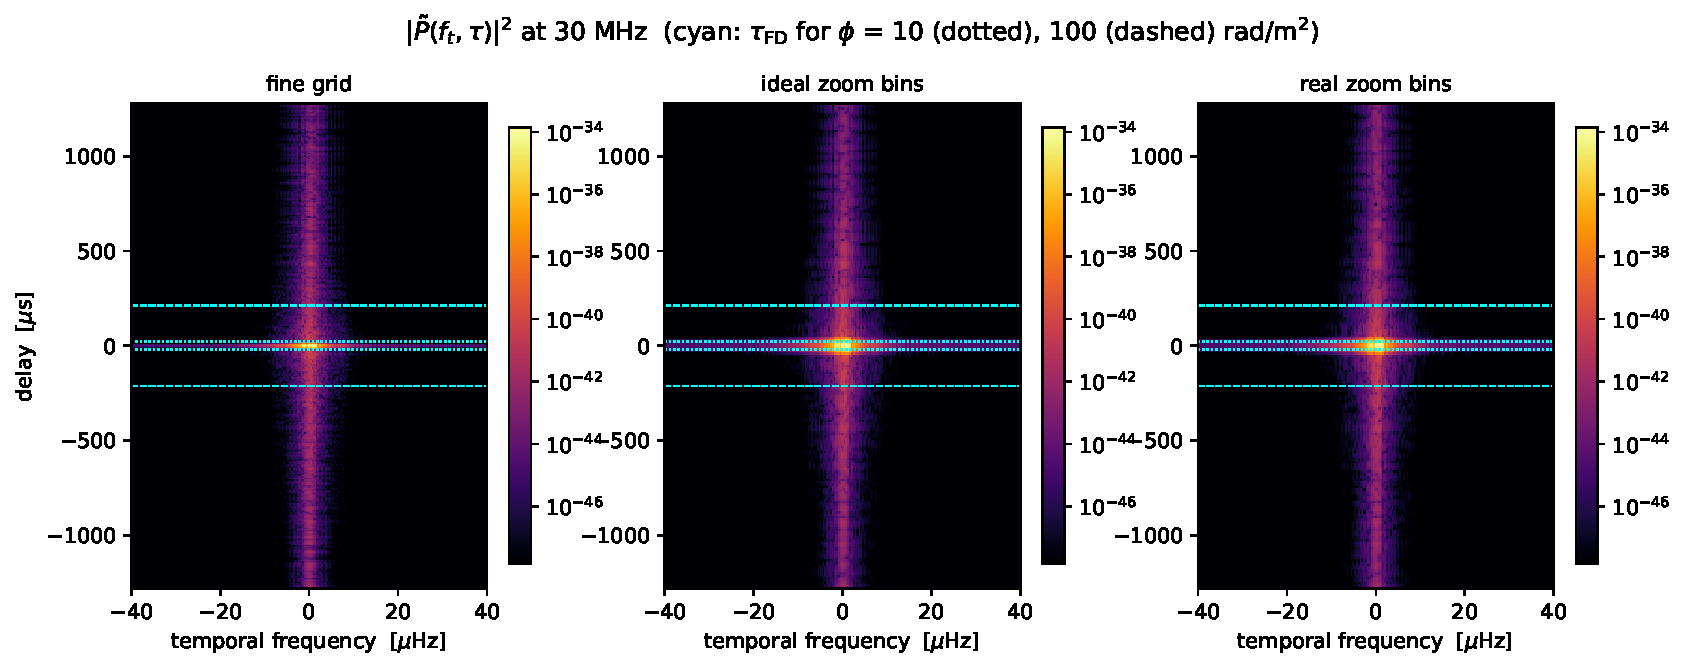
\includegraphics[width=\textwidth]{real30_pspec}
  \caption{2D power spectrum of $\tilde P_{\rm obs} = \Qobs + i\Uobs$
    over (temporal frequency, delay) at 30\,MHz.  With the beam frozen
    in frequency, \emph{all} power at $\tau \neq 0$ is
    Faraday-induced.  The cyan lines mark
    $\tau_{\rm FD} = 2\phi c^2/(\pi\nu^3)$ for
    $\phi = 10, 100\;{\rm rad\,m^{-2}}$.  The real zoom bins (right)
    scatter noticeably more power to high delays than the ideal
    Gaussian bins (middle) — the aliasing artifact floor of the zoom
    channelization.}
  \label{fig:realpspec}
\end{figure}

\section{Step 3: 10 and 50 MHz bands}
\label{sec:bands}

The same analysis was repeated with the band centered at 10 and
50\,MHz (no additional point source: a source is fully degenerate
with a rotation-measure change).  The channel-averaged behaviour
mirrors 30\,MHz — the smooth part of the beam-integrated polarization
is spectrally resolved by every channelization — but the amplitude of
the fast Faraday ``fuzz'' superimposed on it grows dramatically
towards low frequency, as each pixel's oscillation rate scales as
$\nu^{-3}$.

\begin{figure}[htb]
  \centering
  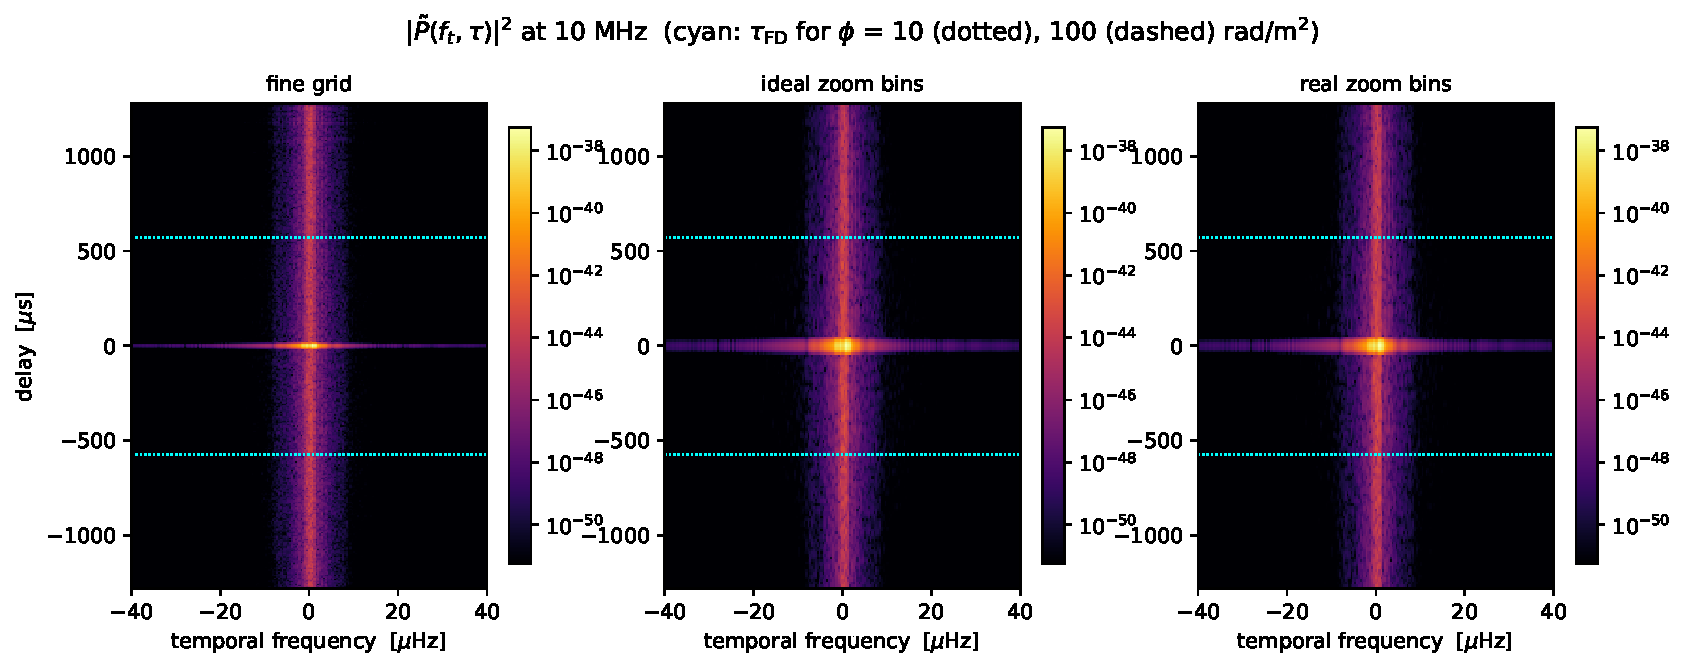
\includegraphics[width=\textwidth]{real10_pspec}
  \caption{As Fig.~\ref{fig:realpspec}, at 10\,MHz.  The Faraday tail
    now fills the entire delay range accessible to the zoom sampling
    ($|\tau| < 1.28$\,ms): at 10\,MHz one ${\rm rad\,m^{-2}}$ of
    Faraday depth corresponds to $57\,\mu$s of delay.}
  \label{fig:pspec10}
\end{figure}

\begin{figure}[htb]
  \centering
  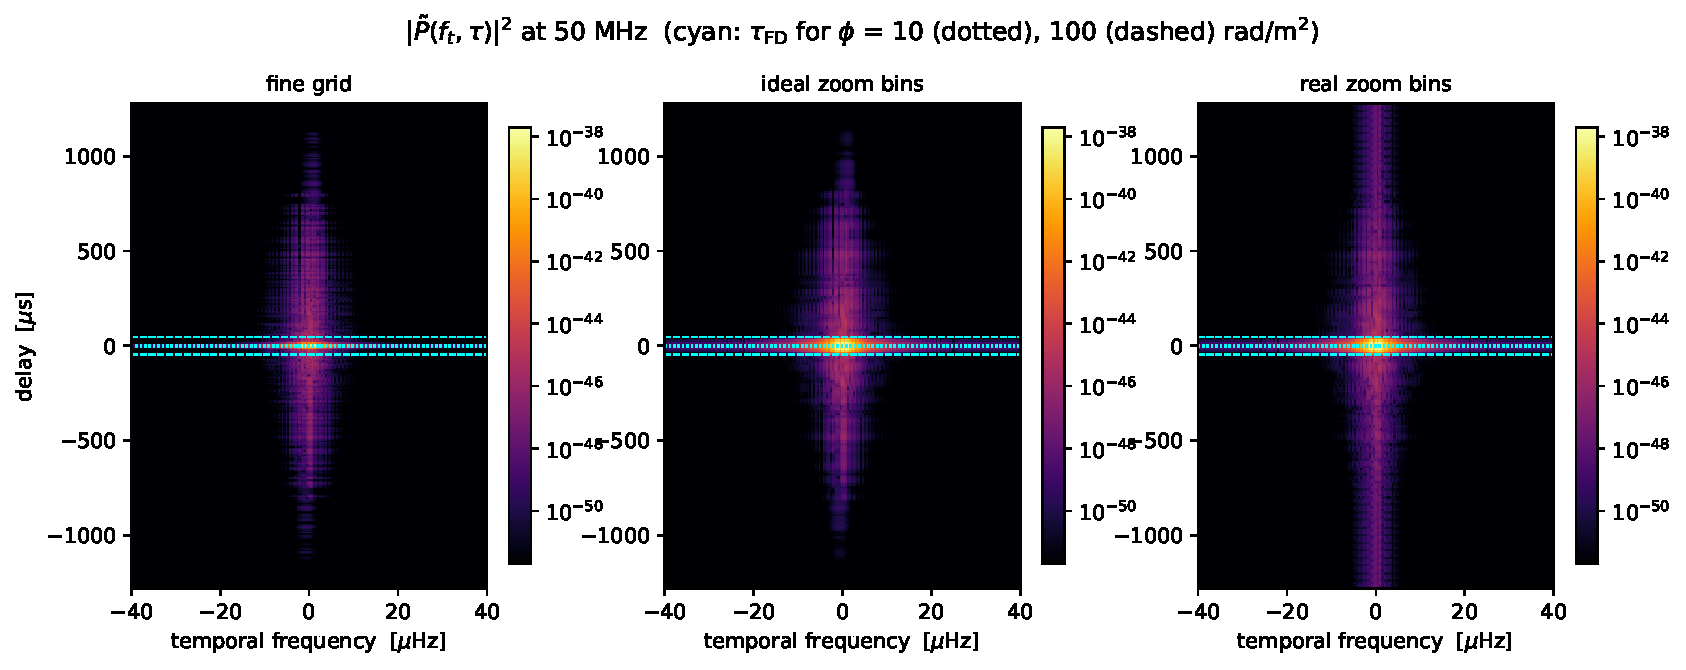
\includegraphics[width=\textwidth]{real50_pspec}
  \caption{As Fig.~\ref{fig:realpspec}, at 50\,MHz.  The Faraday
    signal is confined to a compact ``diamond'' with a sharp edge at
    $|\tau| \simeq 1.1$\,ms — the delay of the largest rotation
    measures on the sky ($|\phi| \simeq 2400\;{\rm rad\,m^{-2}}$ in
    the inner galactic plane).  The real zoom bins (right panel)
    scatter a vertical stripe of aliased power far beyond the true
    envelope, which the ideal Gaussian bins do not.}
  \label{fig:pspec50}
\end{figure}

\section{The perfect-depolarization limit: an I-only sky}
\label{sec:ionly}

How much do the telemetered products actually care about sky
polarization once the Faraday screen has scrambled it?  To answer
this we reran the real-sky simulation with $Q = U = 0$ — the limit of
perfect Faraday depolarization at the band center.  With the frozen
beam and no polarization this sky is exactly frequency-flat, so its
parent bins, zoom bins and fine channels are all identical, and the
comparison against the full run isolates the polarization
contribution to every product.

Two facts emerge.  First, the polarization that \emph{is} observed
through the Faraday screen ($|P_{\rm obs}|/\Iobs \sim 0.15$ at
30\,MHz, cf.\ Fig.~\ref{fig:realsnapshot}) is almost entirely
instrumental leakage of the unpolarized emission: the I-only run
reproduces the 30\,MHz parent-bin
$(\Qobs, \Uobs)/\Iobs = (0.146, -0.032)$ of the full run to within
$2\times10^{-4}$.  (The zenith calibration of Sec.~\ref{sec:unpol}
does not reduce this diffuse-sky leakage — it enforces a single
condition at one direction, while the whole visible hemisphere
contributes here.)  Without the Faraday screen the genuine sky
polarization would contribute a median
$|\Delta P_{\rm obs}|/\Iobs \simeq 6.2\times10^{-2}$ at 30\,MHz; the
beam-scale rotation-measure mixture suppresses this by a factor
$\simeq 380$ in the parent bin.

Second, the residual genuine-polarization signal is
channelization-dependent (Table~\ref{tab:ionly} and
Fig.~\ref{fig:ionlyfrac}).  At 30\,MHz the sky polarization moves the
parent-bin products by a median $1.6\times10^{-4}$ of $\Iobs$ (max
$5.3\times10^{-4}$) and the central zoom bin by $4.5\times10^{-4}$
(max $9.0\times10^{-4}$) — the finer bin averages away less of the
rapidly rotating polarization and retains $\sim 2.7\times$ more of
it.  The contrast is strongest at 10\,MHz (factor $\sim 4$ in
$|\Delta P|$, factor $\sim 5$ in $\Delta I$), where the Faraday
oscillations are fastest, and nearly disappears at 50\,MHz where even
a 25\,kHz bin resolves most of the structure.

\begin{table}[htb]
  \centering
  \caption{Fractional effect of sky polarization on the binned
    products, relative to the perfect-depolarization (I-only) run:
    time-median (max) of $|\Delta X|/\Iobs^{I\,only}$ over one
    sidereal day.}
  \label{tab:ionly}
  \begin{tabular}{lcccc}
    \hline
    & \multicolumn{2}{c}{central parent bin}
    & \multicolumn{2}{c}{central zoom bin} \\
    band & $\Delta I$ & $|\Delta P|$ & $\Delta I$ & $|\Delta P|$ \\
    \hline
    10\,MHz & $7.2\,(18)\times10^{-6}$ & $0.7\,(1.1)\times10^{-4}$
            & $3.8\,(11)\times10^{-5}$ & $2.7\,(5.6)\times10^{-4}$ \\
    30\,MHz & $0.9\,(1.9)\times10^{-4}$ & $1.6\,(5.3)\times10^{-4}$
            & $1.9\,(7.1)\times10^{-4}$ & $4.5\,(9.0)\times10^{-4}$ \\
    50\,MHz & $2.3\,(7.9)\times10^{-4}$ & $2.3\,(9.1)\times10^{-4}$
            & $3.1\,(8.2)\times10^{-4}$ & $3.8\,(10)\times10^{-4}$ \\
    \hline
  \end{tabular}
\end{table}

\begin{figure}[htb]
  \centering
  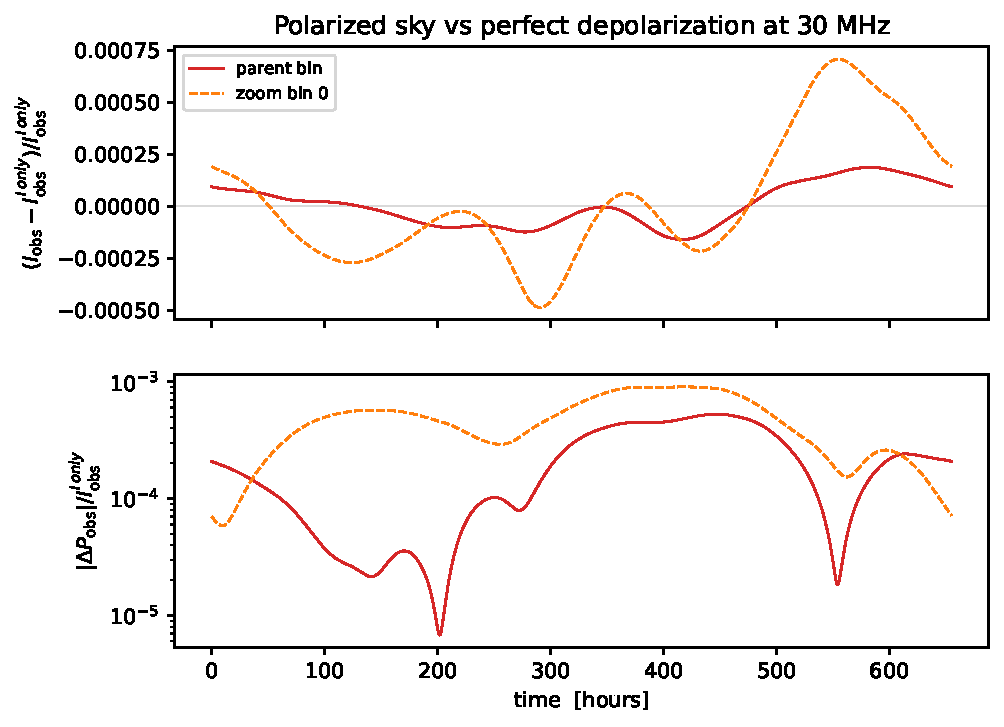
\includegraphics[width=0.85\textwidth]{real30_ionly_frac}
  \caption{Fractional effect of sky polarization at 30\,MHz over one
    sidereal day: intensity shift (top) and polarization shift
    (bottom) of the full-sky run relative to the I-only run, for the
    central parent bin and the central zoom bin.  The zoom bin
    consistently retains a factor of a few more of the
    Faraday-surviving polarization.}
  \label{fig:ionlyfrac}
\end{figure}

For calibration and foreground modeling this is good news twice
over: the total-power products are insensitive to sky polarization at
the few$\times10^{-4}$ level even in the zoom bins, while the
polarization products themselves must be interpreted as
leakage-dominated, with the genuine Faraday-surviving sky signal
accessible only differentially (e.g.\ through the delay-space
statistics of Sec.~\ref{sec:delay}).

\section{Step 4: delay-space signature}
\label{sec:delay}

Because the beam is frozen in frequency, the Faraday screen is the
\emph{only} source of spectral structure, and delay space separates it
cleanly from the (chromatically smooth) sky: a screen of depth $\fd$
maps to the delay
\begin{equation}
  \tau_{\rm FD}(\fd, \nu)
  = \frac{1}{2\pi}\left|\frac{d}{d\nu} 2\fd\lambda^2\right|
  = \frac{2 \fd c^2}{\pi \nu^3}
  \approx 64\,\mu{\rm s}
  \left(\frac{\fd}{30\,{\rm rad\,m^{-2}}}\right)
  \left(\frac{\nu}{30\,{\rm MHz}}\right)^{-3},
\end{equation}
so the ensemble of rotation measures on the sky paints a delay
``spectrum'' that is a beam-weighted image of the RM distribution,
stretched by the steep $\nu^{-3}$ lever arm.

\paragraph{Deconvolving the zoom channelization.}
The zoom stage runs a 64-point FFT on the critically sampled 25\,kHz
parent stream, so each bin has image responses folded about the
parent-band edges: the Nyquist bin ($k = 32$) responds with an exact
50/50 split to the two boundary frequencies $\pm 12.5$\,kHz of its
parent (i.e.\ the slots halfway to each neighboring parent), and the
near-boundary bins retain $\sim 40\%$ images.  Because these response
shapes are known, the mapping from a spectrum gridded on the 192
nominal 390.625\,Hz slots (padded by 32 slots per side to represent
folds from just outside the band) to the 192 measured bins is an
explicit linear transfer matrix — and a well-conditioned one
(condition number 3.9).  We invert it per time sample with a
second-difference (smoothness) regularization, which is needed only
to resolve the degeneracy of the parent-boundary and pad slots that
enter solely through the shared Nyquist folds; a plain min-norm
inverse leaves those few slots free and their errors ring across the
whole delay range.  The result is the ``deconvolved'' curve in
Fig.~\ref{fig:delayprofile}.

\begin{figure}[htb]
  \centering
  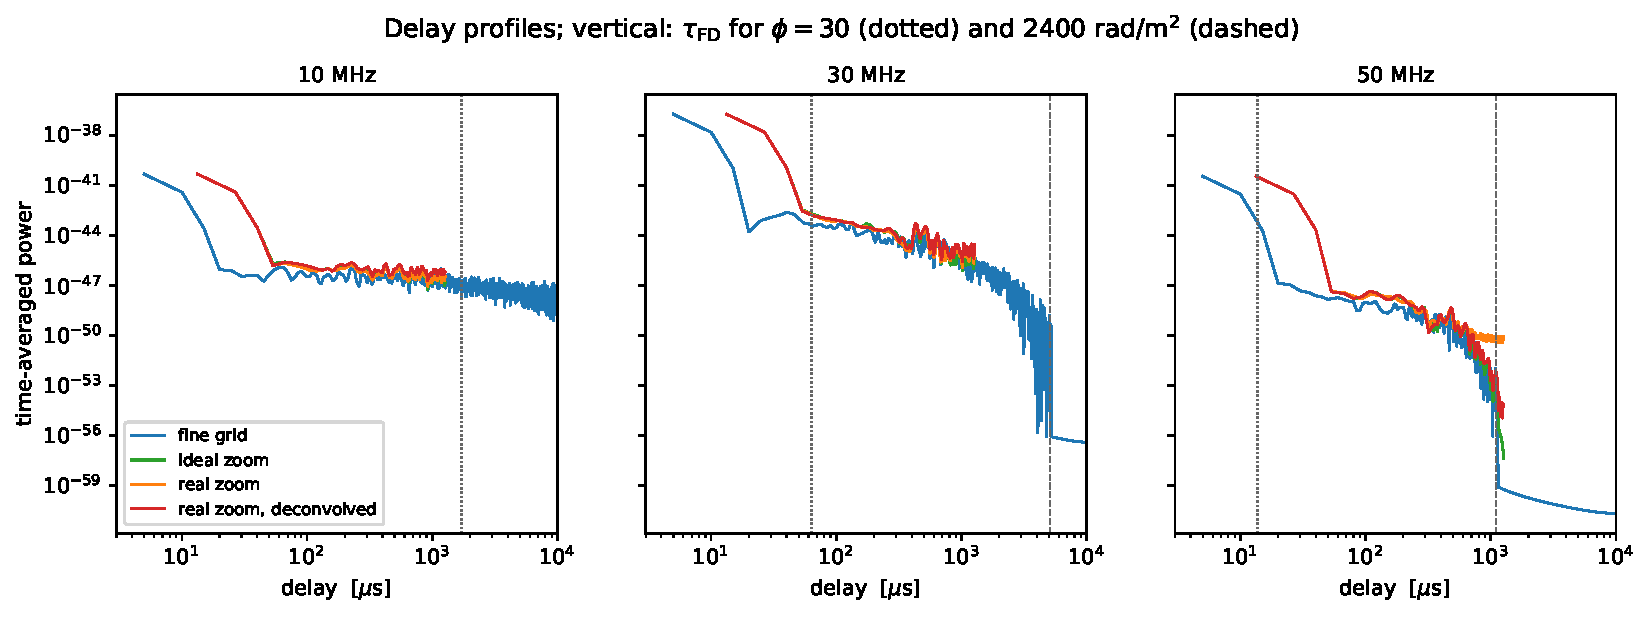
\includegraphics[width=\textwidth]{pspec_delay_profile}
  \caption{Time-averaged delay-power profiles of
    $\tilde P_{\rm obs}$ per band.  The Faraday plateau extends from
    $\tau_{\rm FD}(\phi \sim {\rm few})$ to a sharp cutoff at
    $\tau_{\rm FD}(\phi_{\max} \simeq 2400\;{\rm rad\,m^{-2}})$
    (dashed), clearly visible at 30\,MHz ($\simeq 5$\,ms) and 50\,MHz
    ($\simeq 1.1$\,ms) and beyond the plotted range at 10\,MHz.  The
    zoom bins reproduce the fine-grid profile faithfully between
    $\sim 50\,\mu$s (their leakage-broadened main lobe) and their
    Nyquist delay of 1.28\,ms.  At 50\,MHz the raw \emph{real} zoom
    bins (orange) flatten onto an aliasing floor about three decades
    below the plateau and miss the cutoff, while the ideal Gaussian
    bins keep following the true profile.  The linear deconvolution
    of the known bin transfer (red) removes this floor: it tracks the
    fine-grid profile through the full cutoff, recovering
    $\sim 4$ decades below the raw aliasing floor with the real
    channelizer response.}
  \label{fig:delayprofile}
\end{figure}

Three practical conclusions follow.  (i) The parent 25\,kHz channels
alone cannot reach the Faraday plateau at all: their Nyquist delay of
$20\,\mu$s lies below $\tau_{\rm FD}$ of essentially every line of
sight at $\nu \lesssim 30$\,MHz.  (ii) The 64-fold zoom sampling opens
the window $50\,\mu{\rm s} \lesssim |\tau| \lesssim 1.28$\,ms, which
at 30\,MHz covers rotation measures from $\sim 25$ to
$\sim 600\;{\rm rad\,m^{-2}}$ and at 10\,MHz resolves the ionospheric
regime $\fd \lesssim 20\;{\rm rad\,m^{-2}}$.  (iii) The measured zoom
response aliases $\sim 10^{-3}$ of the strong low-delay power across
the band, but because the bin transfer is known and well conditioned,
a simple regularized linear inversion removes the aliasing floor in
post-processing and restores the ideal-binning performance — at
50\,MHz this is the difference between missing and cleanly resolving
the $\tau_{\rm FD}(\phi_{\max})$ cutoff.

\section{Conclusions}
\label{sec:conclusions}

The four-port LuSEE-Night correlator, propagated through the real
spectrometer channelization, separates Faraday rotation from the
smooth foreground in two complementary regimes.  A bright compact
polarized source (Sec.~\ref{sec:point}) produces coherent
polarization oscillations that the 25\,kHz parent channels erase
(recovered $p \simeq 7\times10^{-4}$ with the leakage-nulled
polarimeter, for $\fd = 250\;{\rm rad\,m^{-2}}$ at 30\,MHz) but the
zoom sub-bins recover at 79--86\% amplitude.  For
the diffuse sky (Secs.~\ref{sec:realsky}--\ref{sec:delay}) the
many-RM mixture within the beam suppresses any single oscillation,
yet the delay-space power spectrum of $\Qobs + i\Uobs$ isolates the
Faraday signal completely: with an achromatic beam all power at
$\tau \neq 0$ is Faraday-induced, its envelope images the sky RM
distribution through $\tau = 2\fd c^2/\pi\nu^3$, and its cutoff
tracks the $\nu^{-3}$ scaling across the 10--50\,MHz bands — a
signature nothing else in the system mimics.  The realistic zoom-bin
response supports this measurement over two decades of delay with an
aliasing floor $\sim 10^{-3}$ of the peak power.

\end{document}
